%%%%%%%%%%%%%%%%%%%%%%%%%%%%%%%%%%%%%%%%%%%%%%%%%%%%%%%%%%%%%%%%%%%%%%%%%%%
%% This file is part of the book
%%
%% Algorithmic Graph Theory
%% http://code.google.com/p/graph-theory-algorithms-book/
%%
%% Copyright (C) 2009, 2010, 2011 Minh Van Nguyen <nguyenminh2@gmail.com>
%%
%% See the file COPYING for copying conditions.
%%%%%%%%%%%%%%%%%%%%%%%%%%%%%%%%%%%%%%%%%%%%%%%%%%%%%%%%%%%%%%%%%%%%%%%%%%%

\documentclass{article}

\usepackage{subfigure}
\usepackage{tikz}
\usetikzlibrary{external}
\tikzexternalize{k-circulant-graphs}

\begin{document}

\begin{figure}
\subfigure[$k = 4$]{
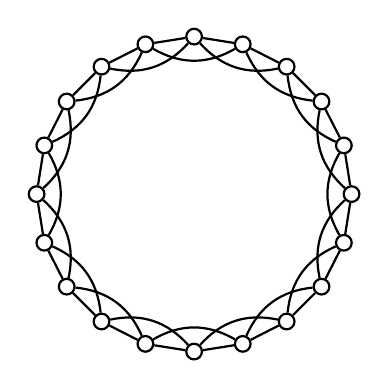
\begin{tikzpicture}
[lineDecorate/.style={-,thick},%
  nodeDecorate/.style={shape=circle,inner sep=2pt,draw,thick},
  scale=2]
%% nodes or vertices
\foreach \nodename/\x/\y in {
  0/1.00000000000000/0.000000000000000,
  1/0.951056516295154/0.309016994374947,
  2/0.809016994374947/0.587785252292473,
  3/0.587785252292473/0.809016994374947,
  4/0.309016994374947/0.951056516295154,
  5/0.000000000000000/1.00000000000000,
  6/-0.309016994374947/0.951056516295154,
  7/-0.587785252292473/0.809016994374947,
  8/-0.809016994374947/0.587785252292473,
  9/-0.951056516295154/0.309016994374947,
  10/-1.00000000000000/0.000000000000000,
  11/-0.951056516295154/-0.309016994374947,
  12/-0.809016994374947/-0.587785252292473,
  13/-0.587785252292473/-0.809016994374947,
  14/-0.309016994374947/-0.951056516295154,
  15/0.000000000000000/-1.00000000000000,
  16/0.309016994374947/-0.951056516295154,
  17/0.587785252292473/-0.809016994374947,
  18/0.809016994374947/-0.587785252292473,
  19/0.951056516295154/-0.309016994374947}
{
  \node (\nodename) at (\x,\y) [nodeDecorate] {};
}
%% edges or lines
\path
\foreach \startnode/\endnode in {
  0/1, 0/19, 1/2, 2/3, 3/4, 4/5, 5/6, 6/7, 7/8, 8/9, 9/10, 10/11,
  11/12, 12/13, 13/14, 14/15, 15/16, 16/17, 17/18, 18/19}
{
  (\startnode) edge[lineDecorate] node {} (\endnode)
}
\foreach \startnode/\endnode in {
  0/2, 1/3, 2/4, 3/5, 4/6, 5/7, 6/8, 7/9, 8/10, 9/11, 10/12, 11/13,
  12/14, 13/15, 14/16, 15/17, 16/18, 17/19, 18/0, 19/1}
{
  (\startnode) edge[lineDecorate,bend left] node {} (\endnode)
};
\end{tikzpicture}
}
%%
%%
\qquad
\subfigure[$k = 6$]{
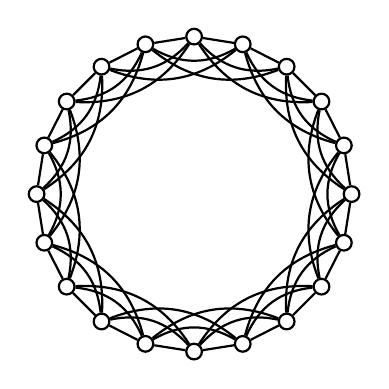
\begin{tikzpicture}
[lineDecorate/.style={-,thick},%
  nodeDecorate/.style={shape=circle,inner sep=2pt,draw,thick},
  scale=2]
%% nodes or vertices
\foreach \nodename/\x/\y in {
  0/1.00000000000000/0.000000000000000,
  1/0.951056516295154/0.309016994374947,
  2/0.809016994374947/0.587785252292473,
  3/0.587785252292473/0.809016994374947,
  4/0.309016994374947/0.951056516295154,
  5/0.000000000000000/1.00000000000000,
  6/-0.309016994374947/0.951056516295154,
  7/-0.587785252292473/0.809016994374947,
  8/-0.809016994374947/0.587785252292473,
  9/-0.951056516295154/0.309016994374947,
  10/-1.00000000000000/0.000000000000000,
  11/-0.951056516295154/-0.309016994374947,
  12/-0.809016994374947/-0.587785252292473,
  13/-0.587785252292473/-0.809016994374947,
  14/-0.309016994374947/-0.951056516295154,
  15/0.000000000000000/-1.00000000000000,
  16/0.309016994374947/-0.951056516295154,
  17/0.587785252292473/-0.809016994374947,
  18/0.809016994374947/-0.587785252292473,
  19/0.951056516295154/-0.309016994374947}
{
  \node (\nodename) at (\x,\y) [nodeDecorate] {};
}
%% edges or lines
\path
\foreach \startnode/\endnode in {
  0/1, 0/19, 1/2, 2/3, 3/4, 4/5, 5/6, 6/7, 7/8, 8/9, 9/10, 10/11,
  11/12, 12/13, 13/14, 14/15, 15/16, 16/17, 17/18, 18/19}
{
  (\startnode) edge[lineDecorate] node {} (\endnode)
}
\foreach \startnode/\endnode in {
  0/2, 0/3, 1/3, 1/4, 2/4, 2/5, 3/5, 3/6, 4/6, 4/7, 5/7, 5/8, 6/8,
  6/9, 7/9, 7/10, 8/10, 8/11, 9/11, 9/12, 10/12, 10/13, 11/13, 11/14,
  12/14, 12/15, 13/15, 13/16, 14/16, 14/17, 15/17, 15/18, 16/18,
  16/19, 17/0, 17/19, 18/0, 18/1, 19/1, 19/2}
{
  (\startnode) edge[lineDecorate,bend left] node {} (\endnode)
};
\end{tikzpicture}
}
%%
%%
\qquad
\subfigure[$k = 8$]{
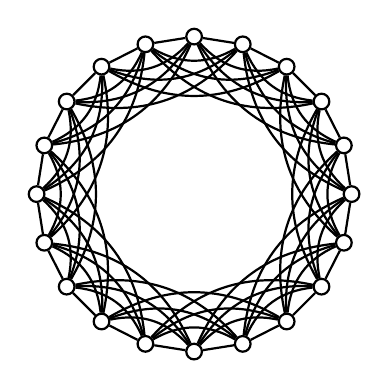
\begin{tikzpicture}
[lineDecorate/.style={-,thick},%
  nodeDecorate/.style={shape=circle,inner sep=2pt,draw,thick},
  scale=2]
%% nodes or vertices
\foreach \nodename/\x/\y in {
  0/1.00000000000000/0.000000000000000,
  1/0.951056516295154/0.309016994374947,
  2/0.809016994374947/0.587785252292473,
  3/0.587785252292473/0.809016994374947,
  4/0.309016994374947/0.951056516295154,
  5/0.000000000000000/1.00000000000000,
  6/-0.309016994374947/0.951056516295154,
  7/-0.587785252292473/0.809016994374947,
  8/-0.809016994374947/0.587785252292473,
  9/-0.951056516295154/0.309016994374947,
  10/-1.00000000000000/0.000000000000000,
  11/-0.951056516295154/-0.309016994374947,
  12/-0.809016994374947/-0.587785252292473,
  13/-0.587785252292473/-0.809016994374947,
  14/-0.309016994374947/-0.951056516295154,
  15/0.000000000000000/-1.00000000000000,
  16/0.309016994374947/-0.951056516295154,
  17/0.587785252292473/-0.809016994374947,
  18/0.809016994374947/-0.587785252292473,
  19/0.951056516295154/-0.309016994374947}
{
  \node (\nodename) at (\x,\y) [nodeDecorate] {};
}
%% edges or lines
\path
\foreach \startnode/\endnode in {
  0/1, 0/19, 1/2, 2/3, 3/4, 4/5, 5/6, 6/7, 7/8, 8/9, 9/10, 10/11,
  11/12, 12/13, 13/14, 14/15, 15/16, 16/17, 17/18, 18/19}
{
  (\startnode) edge[lineDecorate] node {} (\endnode)
}
\foreach \startnode/\endnode in {
  0/2, 0/3, 0/4, 1/3, 1/4, 1/5, 2/4, 2/5, 2/6, 3/5, 3/6, 3/7, 4/6,
  4/7, 4/8, 5/7, 5/8, 5/9, 6/8, 6/9, 6/10, 7/9, 7/10, 7/11, 8/10,
  8/11, 8/12, 9/11, 9/12, 9/13, 10/12, 10/13, 10/14, 11/13, 11/14,
  11/15, 12/14, 12/15, 12/16, 13/15, 13/16, 13/17, 14/16, 14/17,
  14/18, 15/17, 15/18, 15/19, 16/0, 16/18, 16/19, 17/0, 17/1, 17/19,
  18/0, 18/1, 18/2, 19/1, 19/2, 19/3}
{
  (\startnode) edge[lineDecorate,bend left] node {} (\endnode)
};
\end{tikzpicture}
}
\end{figure}

\end{document}
